
Joining the AJFS system requires knowing the hostname and port of at least one
active node in the system. Joining is a two-phase process. For convenience, we
denote the new node wishing to join the group the "joiner", and the active node
that the joiner knows about is the "facilitator".

Figure \ref{fig:algorithm} describes the join procedure of AJFS server. The joiner starts off by sending a \texttt{requestJoinLock()} RPC request to the
facilitator. The facilitator then ensures that no files are open for writing,
and then attempts to lock all of the hosts in the AJFS system using the
\texttt{getJoinLock()} RPC. If the facilitator is not able to get the "join
lock" from all other hosts, or if files are open for writing, it will return to
the joiner that it failed, and the joiner must try again at a later time.

If the facilitator is able to get a join lock from every other node in the
system, it returns back to the joiner that the request succeeded as well as the
absolute path on the facilitator for the facilitator's local database.

At this point, the joiner \texttt{rsync}s its own local database with the
database on the facilitator. \texttt{rsync} was chosen because it is fairly
efficient, is already available, and allows a brand new host that has never
joined before to join using the same procedure as a node that has previously
failed and is coming back.

When the joiner has finished \texttt{rsync}ing, it must start up all necessary
worker threads, and then send a \texttt{join()} RPC to the facilitator. The
facilitator in turn calls \texttt{addServer()} on all of the other nodes,
passing to them the information needed to contact the joiner. Afterwards, it
calls \texttt{releaseJoinLock()} on all of the servers. Finally, it then returns
to the new joiner the list of other hosts that the facilitator knows are in the
system.

In order for this to be safe, several properties have to hold. When a node 
holds the "join lock", no additional modifications to the file system can
proceed. As a result, local operations must block until the "join lock" is
released. Similarly, the joiner must not make any changes to its own file system
until after \texttt{join()} returns.

To be robust to failures of both the joiner and the facilitator, the "join
locks" must be able to timeout. This process is described in
Section~\ref{sec:hostManager}. A node is fully "alive" only once
\texttt{releaseJoinLock()} has been called on \textbf{all} other live servers.
If any call fails, the joining server will eventually been told that it must
rejoin by the node whose \texttt{releaseJoinLock()} was not called.

\begin{figure}[Ht]
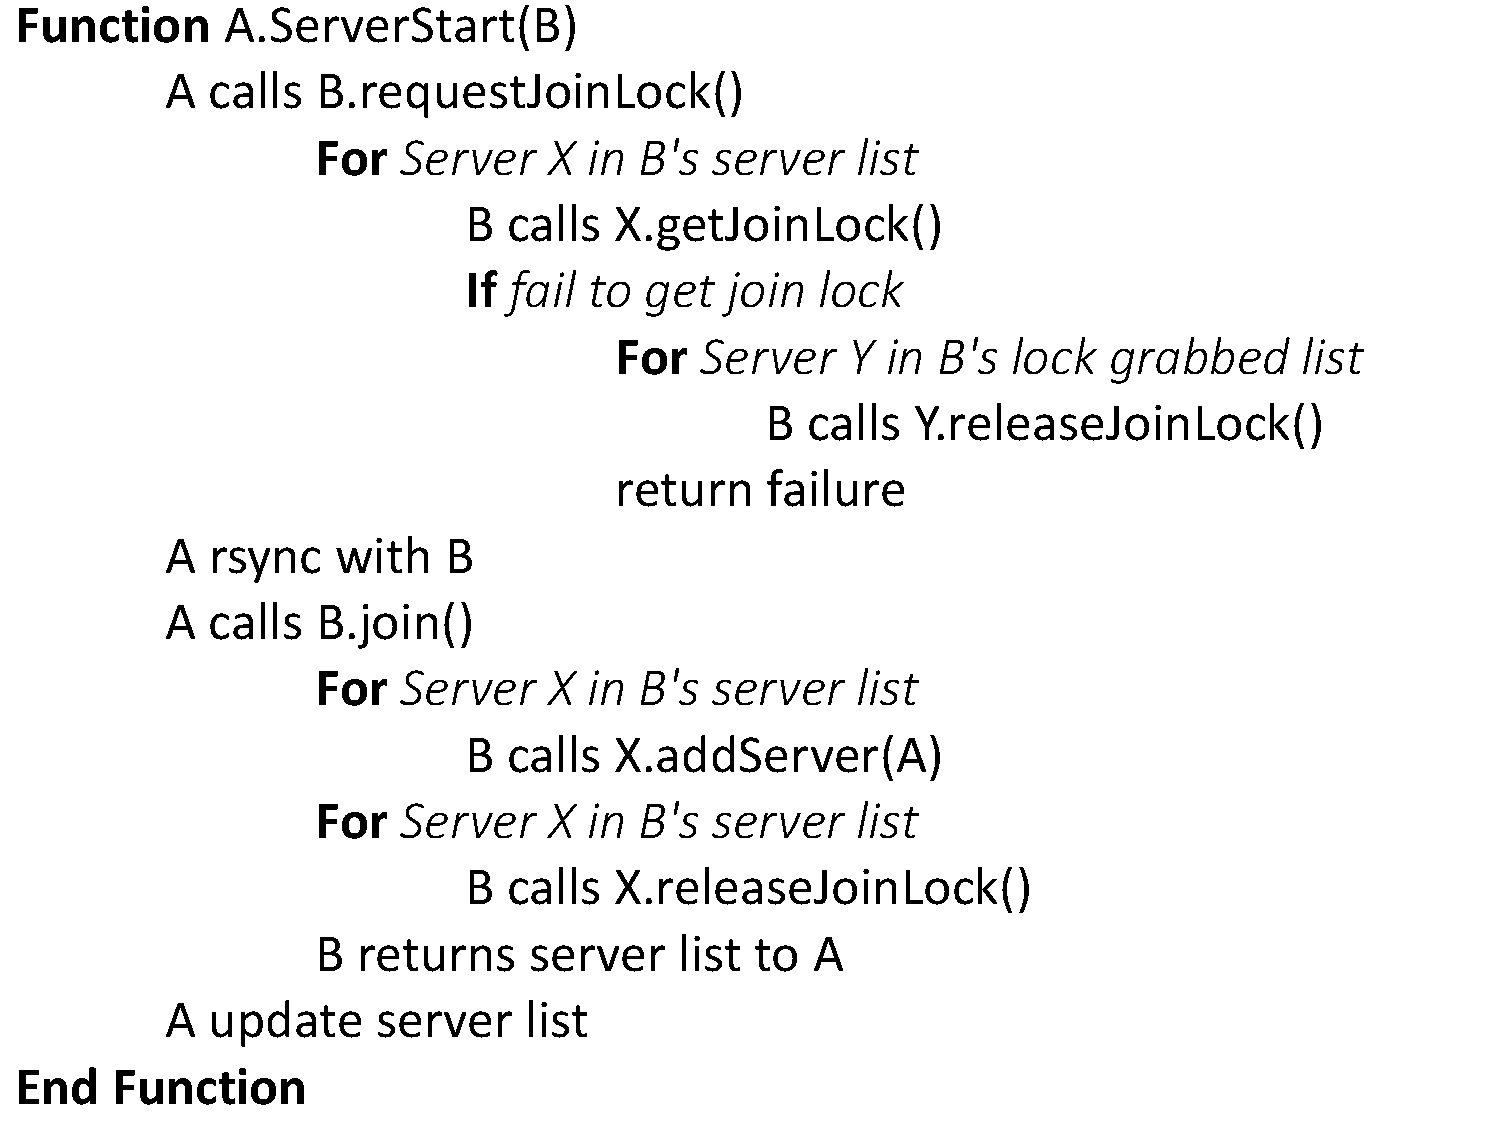
\includegraphics[width=\linewidth]{algorithm.pdf}
\caption{Pseudo-code for AJFS server join}
\label{fig:algorithm}
\vspace{-5mm}
\end{figure}

%\begin{algorithm}
%\caption{\figtitle{Pseudo-code for AJFS join procedure}}
%\label{algo:joinProcedure} 

%\begin{algorithmic}

%\Function{A.ServerStart with B as remote host}{\null}
%\State A calls B.requestJoinLock()
%	\For{Server X in B's server list}
%		\State B calls X.getJoinLock()
%		\If{$fail\ to\ get\ join\ lock$}
%			\For{Server Y in B's lock grabbed list}
%				\State B calls Y.releaseJoinLock()
%				\State return failure
%		\EndIf
%	\EndFor
%\State A rsync with B
%\State A calls B.join()
%	\For{Server X in B's server list}
%		\State B calls X.addServer(A)
%	\EndFor
%	\For{Server X in B's server list}
%		\State B calls X.releaseJoinLock()
%	\EndFor
%	\State B returns server list to A
%\State A update server list
%\EndFunction
%\end{algorithmic}
%\end{algorithm} 
